\documentclass[10pt]{beamer}

\usetheme[progressbar=frametitle]{metropolis}
\usepackage{appendixnumberbeamer}

\usepackage{booktabs}
\usepackage[scale=2]{ccicons}

\usepackage{pgfplots}
\usepgfplotslibrary{dateplot}
\usepackage{comment}
\usepackage{xspace}
\usepackage{graphicx} 
\usepackage{subcaption}
\usepackage{subcaption}

\newcommand{\themename}{\textbf{\textsc{metropolis}}\xspace}

\title{Segment and test approach on transport for hamiltonian systems}
\date{\today}
%\date{}
\author{André Farinha Bósio$^{1,2}$, Yves Elskens$^{2}$, Iberê Luiz Caldas$^{1}$}
\institute{$^1$Universidade de São Paulo - Brazil\\ $^2$Aix-Marseille Université - France}
\titlegraphic{
\hfill
\includegraphics[height=1cm]{if.png}
\hfill
\includegraphics[height=1cm]{Identidade_Visual_CAPES.png}
\hfill
\includegraphics[height=1cm]{aix.jpg}
\hfill
\includegraphics[height=1cm]{piim.png}
\hfill
\includegraphics[height=1cm]{mesocentre.png}
\hfill
\includegraphics[height=1cm]{Logo-CNRS.png}

}



%\usepackage[brazilian]{babel}
\usepackage[english]{babel}

\begin{document}

\maketitle






\begin{frame}{What is transport?}
\begin{itemize}
    \item How things, such as heat and mass, spread over time:
\end{itemize}

\begin{columns}[t]
    \begin{column}{0.5\textwidth}
    \begin{figure}
        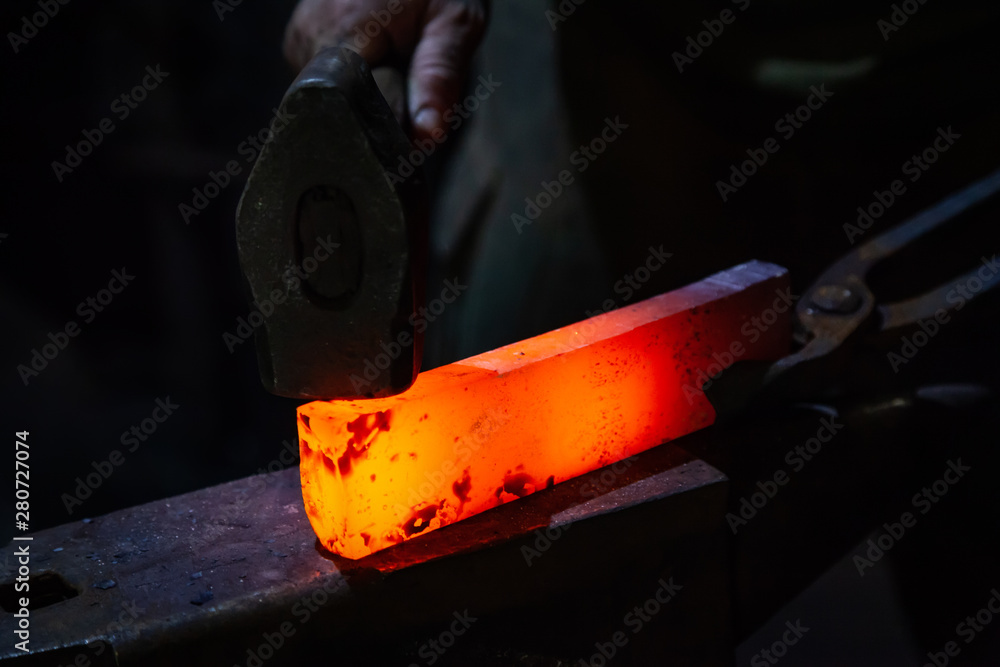
\includegraphics[height = 2cm]{imgs/heat.jpg}
        \caption*{\textbf{normal}, such as heat in a metal bar}
    \end{figure}    
    

    \end{column}
    \begin{column}{0.5\textwidth}
        \begin{figure}
            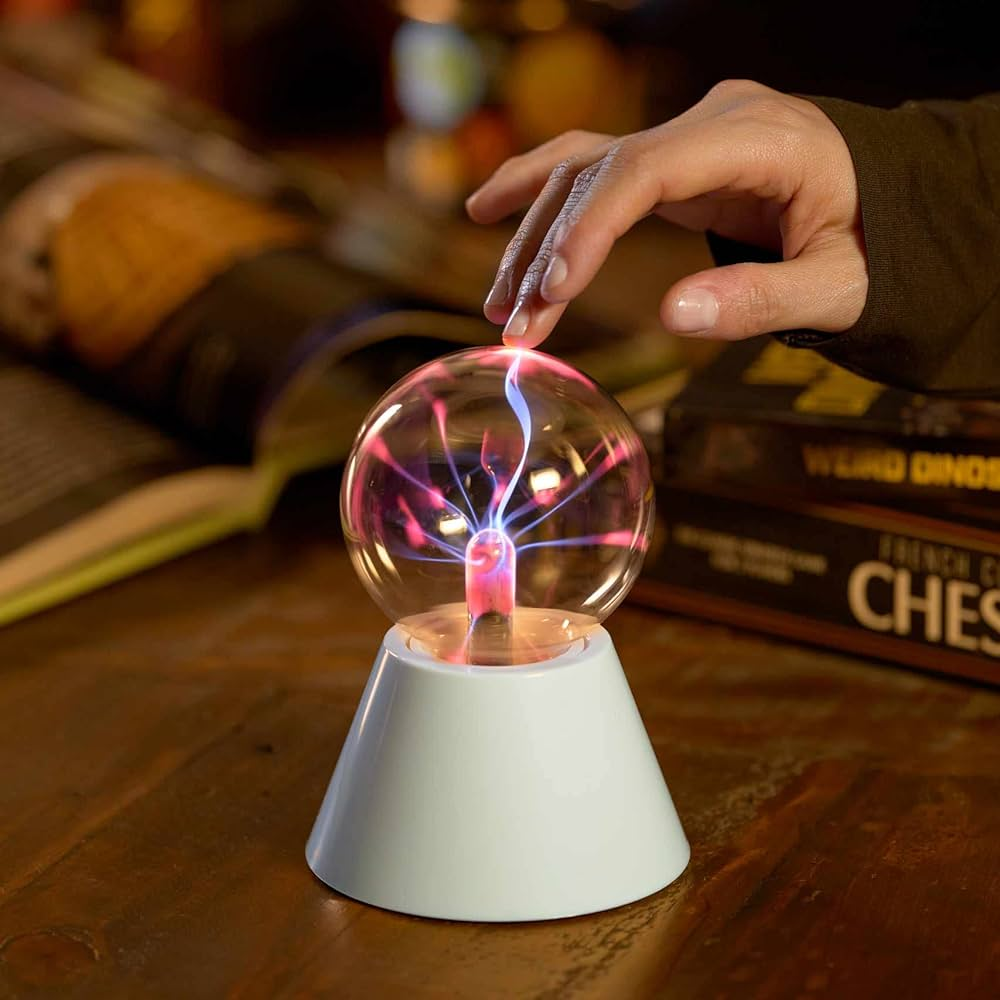
\includegraphics[height = 2cm]{imgs/plasma.jpg}
            \caption*{\textbf{anomalous}, as it is in some plasmas}
        \end{figure}   
    \end{column}
    
\end{columns}
One tool to characterize transport is with the behavior of a power law of the mean square displacement: $\sigma(t)^2 = Ct^\gamma$
\begin{figure}[l]
    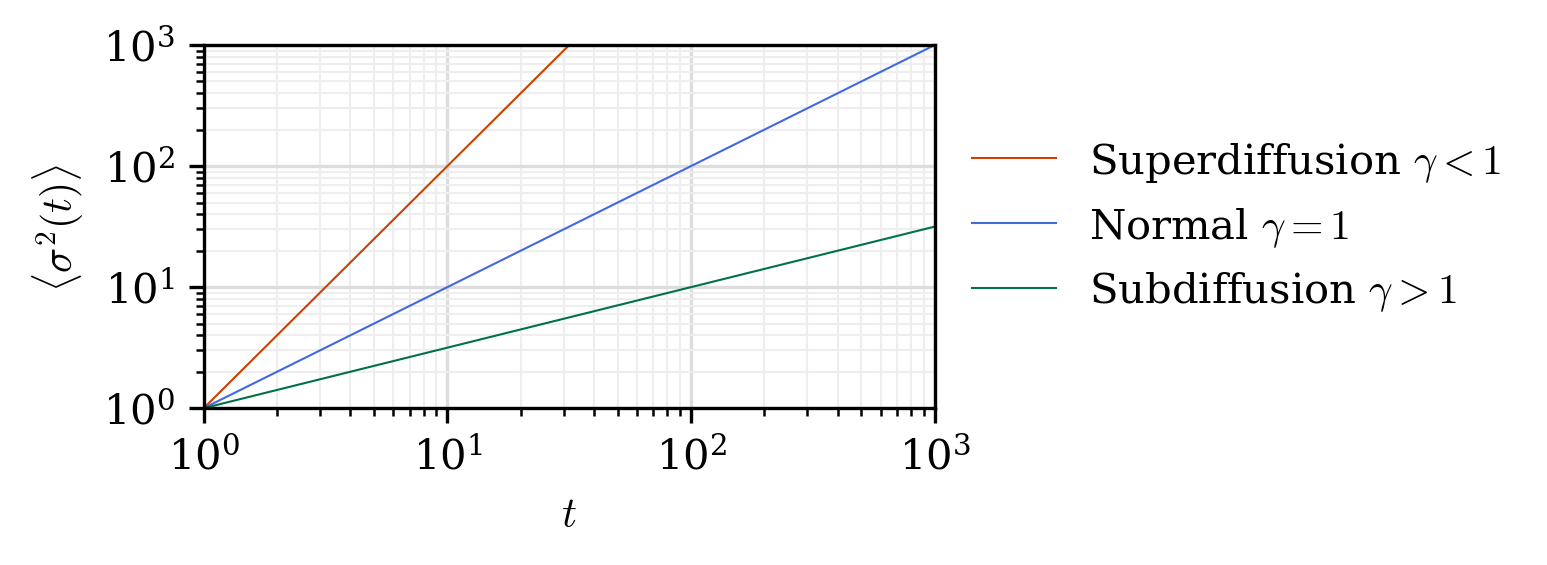
\includegraphics[height = 3cm]{other/graph.png}
\end{figure}



\end{frame}


\begin{frame}{Segment and test - Why and How}
    \textbf{Why} do it?
    \begin{itemize}
        \item Evaluation of $\gamma$ is expensive, requiring thousands of initial condition iterated over long times
        \item Ballistic modes are sufficient condition for anomalous transport
    \end{itemize}

    \textbf{What} is it?
    \begin{itemize}
        \item Fast method to identify anomalous transport trough the existence of ballistic modes
        \item Tunable parameters 
        \item Around 10 times, cheaper compared to usual methods
    \end{itemize}

    \textbf{How} do it?
    \begin{enumerate}
        \item Pick some initial conditions $\approx 100$
        \item Create the Poincaré section
        \item Separate regions with image processing
        \item Test the regime in each region
    \end{enumerate}



\end{frame}



\begin{frame}{Segment and test - Example}
    We can test the method on the standard map:
    $$  p_{n+1} = p_n + K\sin(\theta_n) \hspace{0.1cm},\hspace{0.1cm} \theta_{n+1} = \theta_n + p_{n+1} \hspace{0.1cm} \textnormal{mod}(2\pi) $$
    
   \hline
    \begin{columns}[t]
        
        \begin{column}{0.5\textwidth}
        
        \begin{figure}
            \begin{subfigure}[t]{0.4\textwidth}
                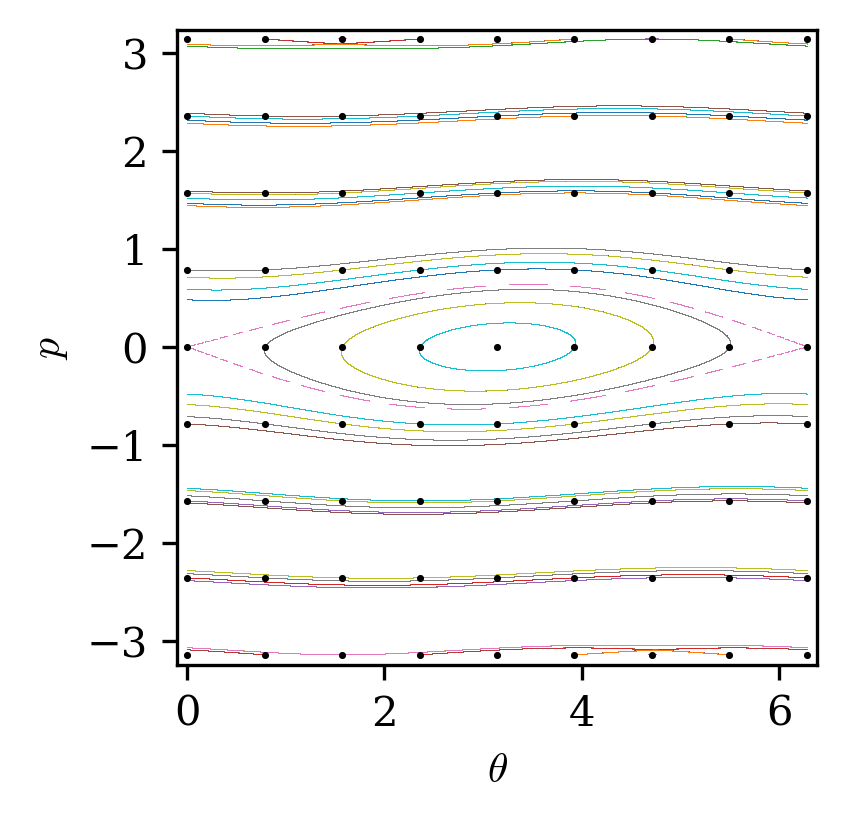
\includegraphics[width=\textwidth]{std/map_1_0.1000.png}
                \caption*{$K = 0.1$; $\gamma = 0$}
            \end{subfigure}
            \begin{subfigure}[t]{0.4\textwidth}
                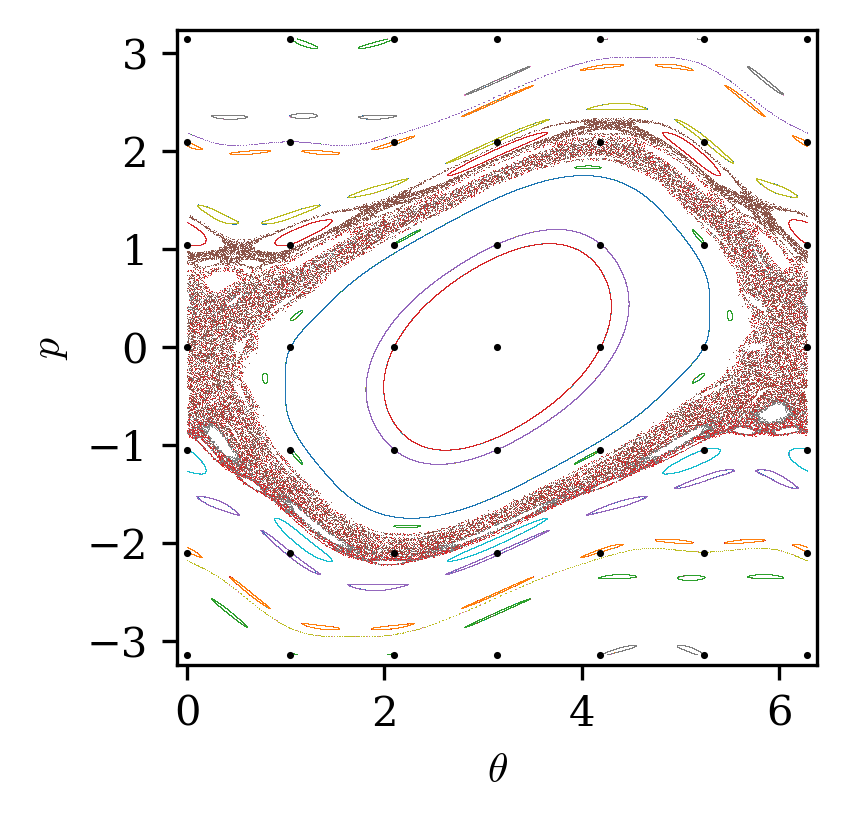
\includegraphics[width=\textwidth]{std/map_1_0.9000.png}
                \caption*{$K = 0.9$; $\gamma = 0$}
            \end{subfigure}
            \begin{subfigure}[t]{0.4\textwidth}
                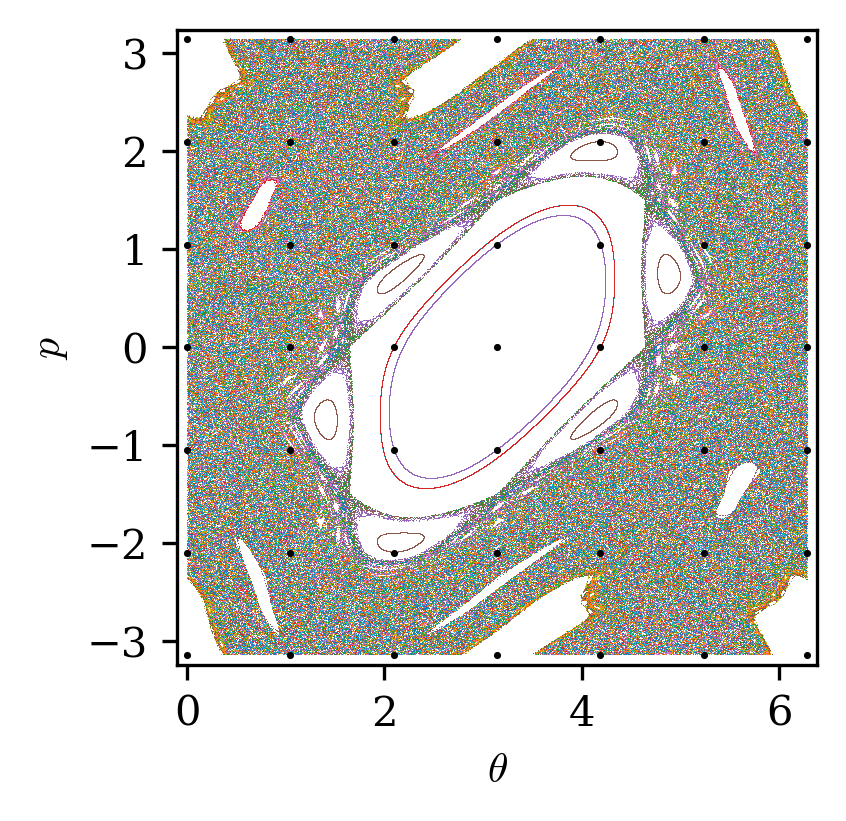
\includegraphics[width=\textwidth]{std/map_1_1.5000.png}
                \caption*{$K = 1.5$; $\gamma = 1$}
            \end{subfigure}
            \begin{subfigure}[t]{0.4\textwidth}
                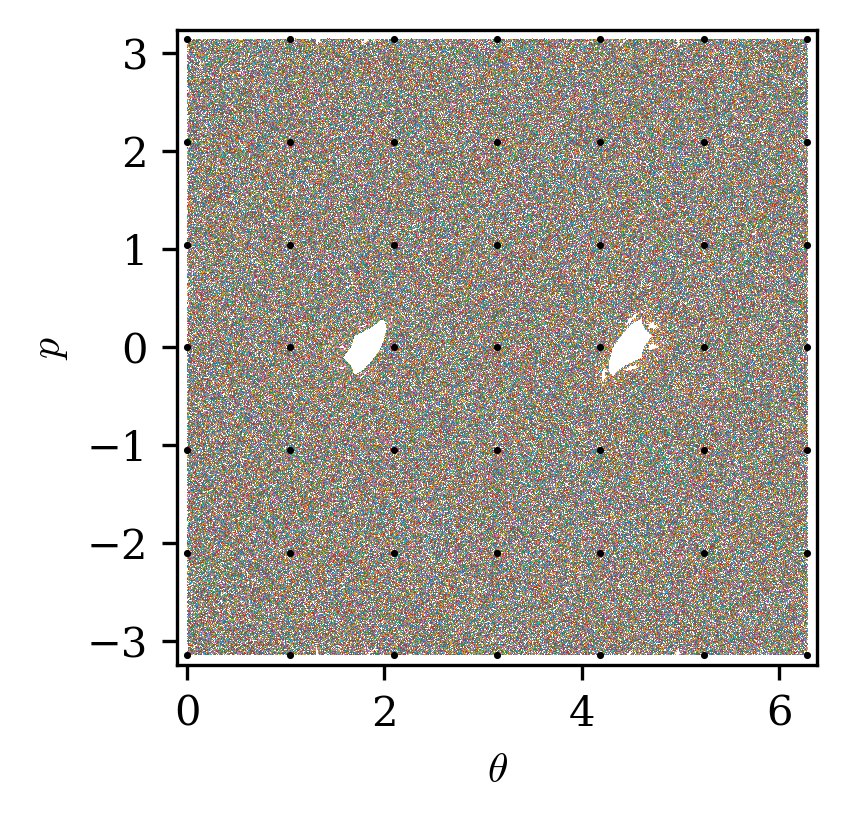
\includegraphics[width=\textwidth]{std/map_1_6.5000.png}
                \caption*{$K = 6.5$; $\gamma > 1$}
            \end{subfigure}
            \caption*{How the map changes with $K$}
        \end{figure}
        
        \end{column}

        

        \begin{column}{0.5\textwidth}
            \begin{figure}
                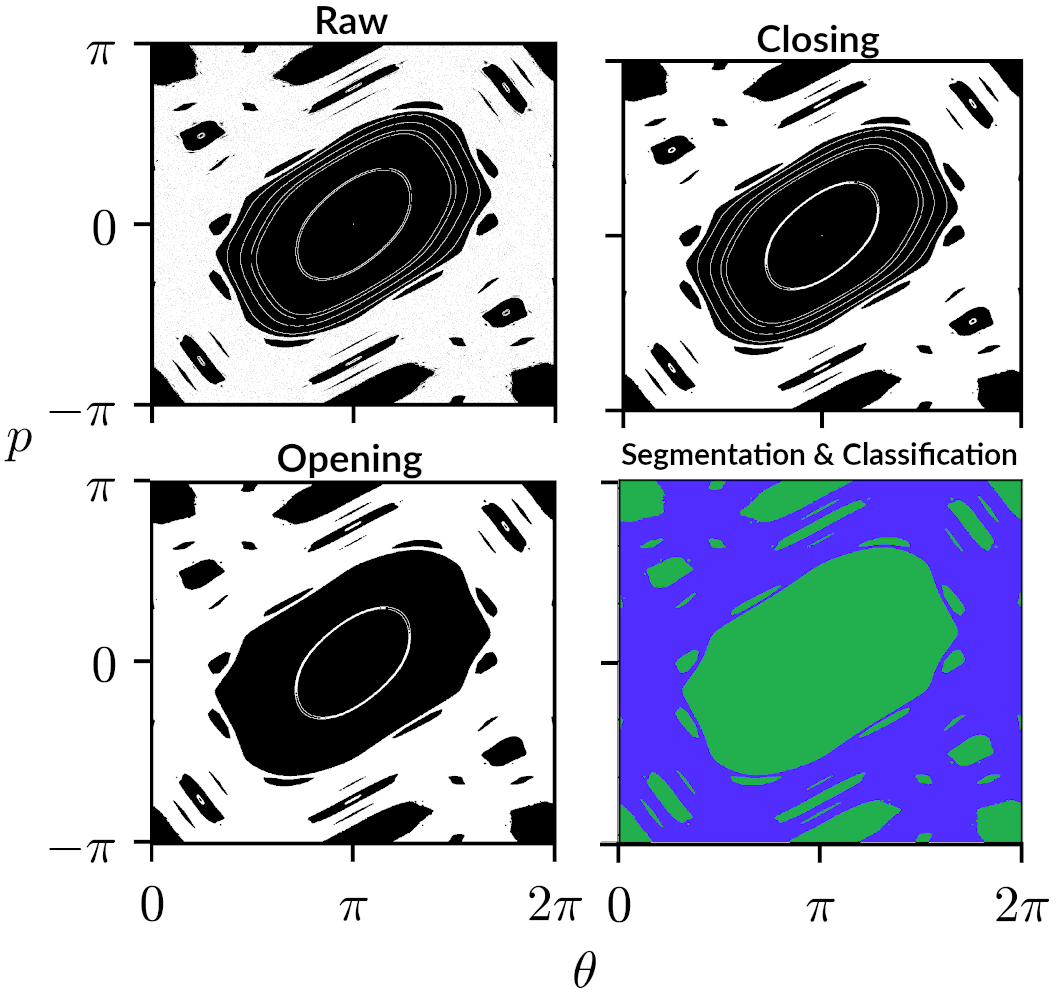
\includegraphics[height = 5cm]{std/mix.png}
                \caption*{Example of the method}
            \end{figure}   
        \end{column}
        
    \end{columns}

\end{frame}



\begin{frame}{Continuous time system - The actual problem}
    \begin{equation*}
        H(x,y,t) = \phi_o - v_1x + A_1 \sin(k_{x1}x)\cos(k_{y1}y) + {A_2}\sin(k_{x2}x + \theta_x)\cos(k_{y2}(y - v\underset{\uparrow}{t})).
      \end{equation*}
    
  
    \begin{figure}
        \begin{subfigure}[b]{0.45\textwidth}
            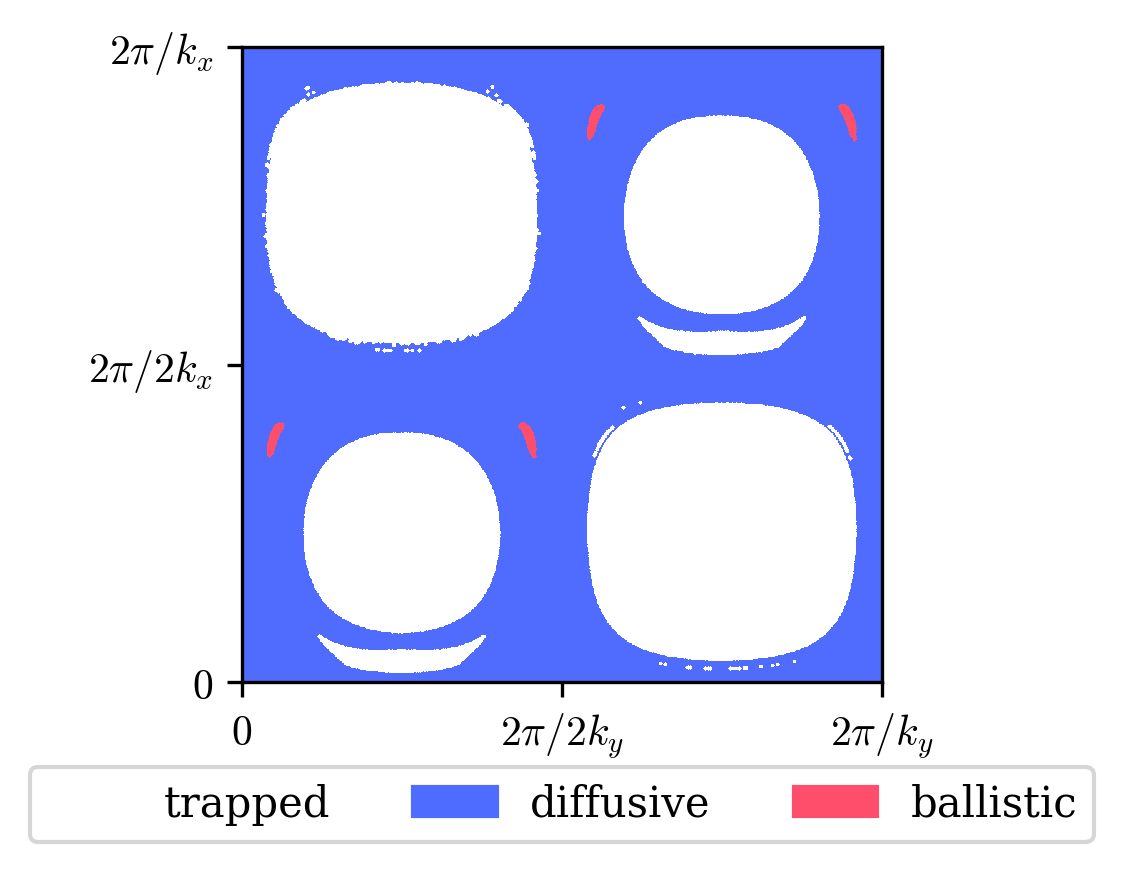
\includegraphics[width=\textwidth]{graf_2ondas/000.1600_000.7854.png}
            \caption{$A_2 = 0.16$}
        \end{subfigure}
        \begin{subfigure}[b]{0.45\textwidth}
            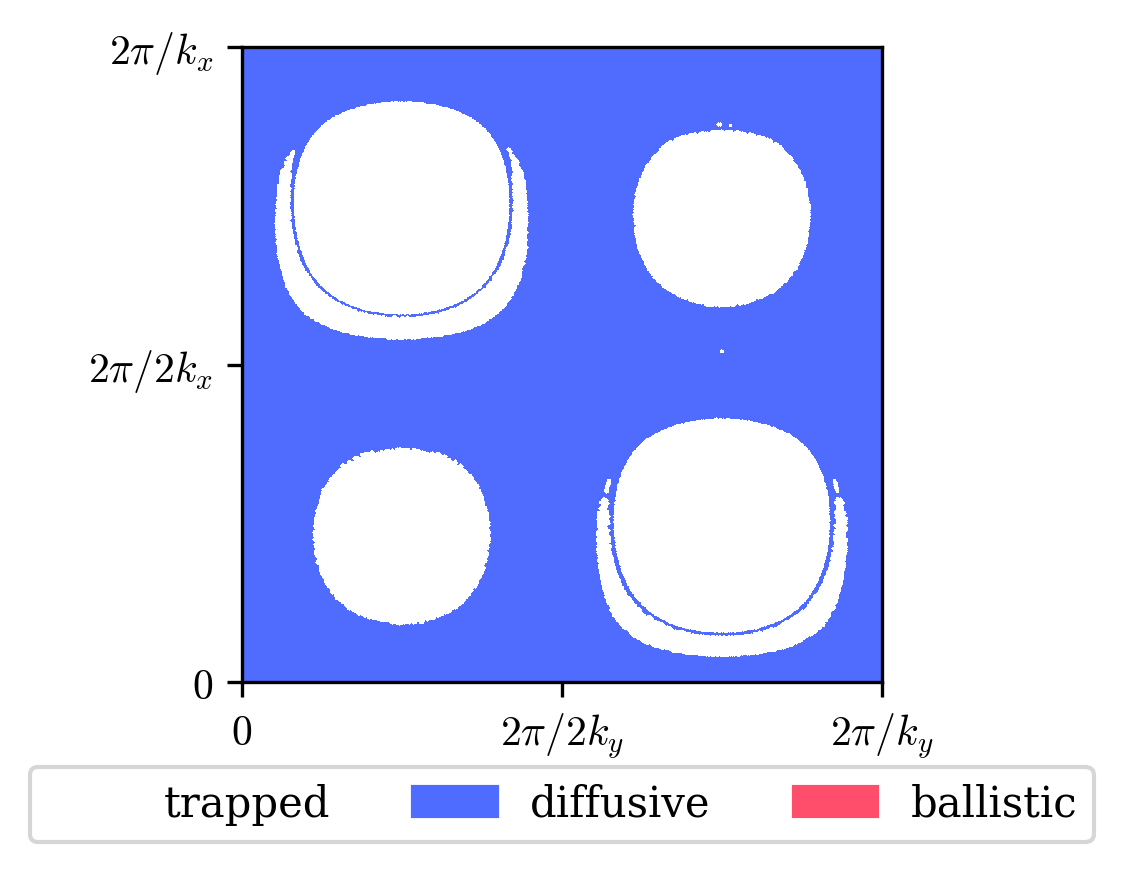
\includegraphics[width=\textwidth]{graf_2ondas/000.2100_000.7854.png}
            \caption{$A_2 = 0.2$}
        \end{subfigure}
        \caption{Categorization on the two wave system. $\theta_x = \frac{\pi}{4}$.}
    \end{figure}
\end{frame}


\begin{frame}

\begin{center}
    {\huge  Thank you \\ \\ See you at the poster}
    \begin{figure}
        \includegraphics{}
    \end{figure}

\end{center}
\end{frame}

\begin{frame}{Extras - Morphology}

    \centering
    \begin{figure}
        
        \begin{subfigure}[b]{0.3\textwidth}
            
\includegraphics[height = 2cm]{imgs/j.png}
            \caption{Referene}
        \end{subfigure}
        \begin{subfigure}[b]{0.3\textwidth}
            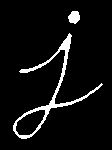
\includegraphics[height = 2cm]{imgs/erosion.png}
            \caption{Erosion}
        \end{subfigure}
        \begin{subfigure}[b]{0.3\textwidth}
            
\includegraphics[height = 2cm]{imgs/dilation.png}
            \caption{Dilation}
        \end{subfigure}
    \caption{Basic Operations}
    \end{figure}

    \begin{figure}
        \begin{subfigure}[b]{0.25\textwidth}
            
\includegraphics[height = 2cm]{imgs/closing.png}
            \caption{Closing}
        \end{subfigure}\hspace{1cm}
        \begin{subfigure}[b]{0.25\textwidth}
            
\includegraphics[height = 2cm]{imgs/opening.png}
            \caption{Opening}
        \end{subfigure}
        \caption{Filtering operations}
    \end{figure}






\end{frame}

\begin{frame}{Extras - Where standard map appears}
    \begin{itemize}
        \item On mechanics: periodically kicked rotor
        \item On particle wave interaction: accelerators
        \item Numerical integration of the a pendulum
    \end{itemize}

    \begin{figure}
        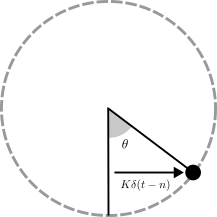
\includegraphics[width = 0.33\textwidth]{imgs/rotor.png}
        \caption{Kicked rotor}
    \end{figure}

\end{frame}

\begin{frame}{Extras - What is a Poincaré section}

    \begin{figure}
        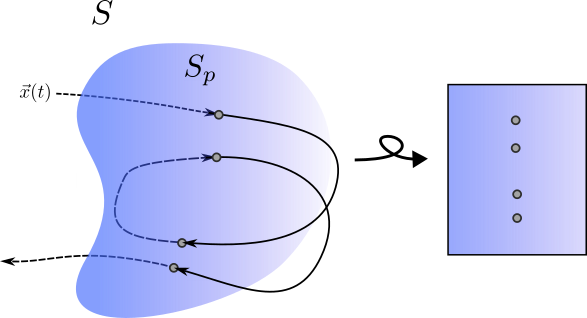
\includegraphics[width = 0.75\textwidth]{imgs/Poincare_map.svg.png}
        \caption{Visual representation of a Poincaré section}
    \end{figure}
\end{frame}

\begin{frame}{Extras - Regimes standard map}
    \begin{figure}
        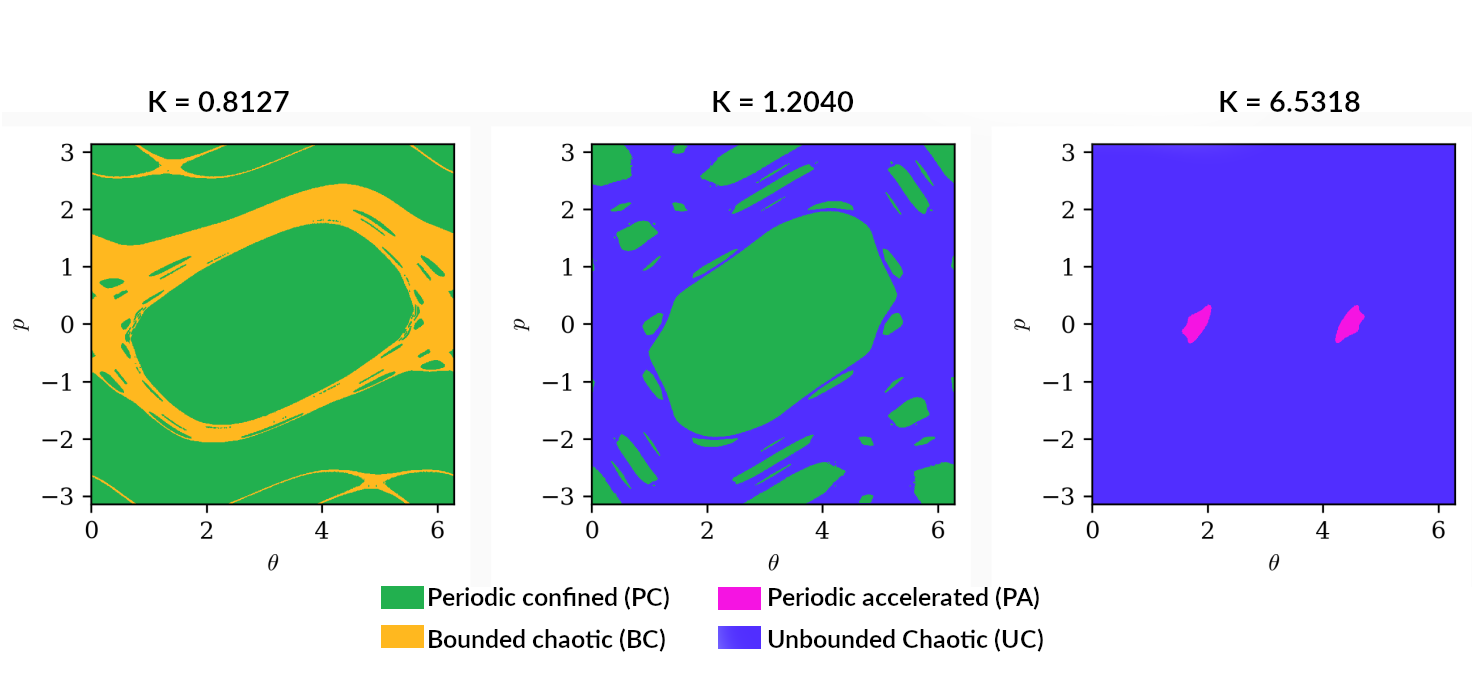
\includegraphics[width = 0.75\textwidth]{std/types.png}
        \caption{The different regimes of the standard map}
    \end{figure}
\end{frame}

\begin{frame}{Extras - Methods comparison}
    \begin{figure}
        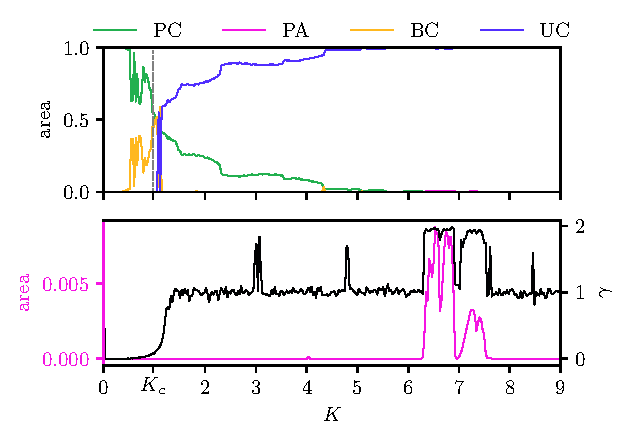
\includegraphics[width = 0.75\textwidth]{std/areas.pdf}
        \caption{Existence of anomalous transport when accelerator modes are present}
    \end{figure}
\end{frame}


\begin{frame}{Extras - continuous time system - flights}
    \begin{equation}
        H(x,y,t) = \phi_o - v_1x + A_1 \sin(k_{x1}x)\cos(k_{y1}y) + {A_2}\sin(k_{x2}x + {\theta_x})\cos(k_{y2}(y - vt)).
      \end{equation}
    

    \begin{figure}
        \begin{subfigure}[b]{0.45\textwidth}
            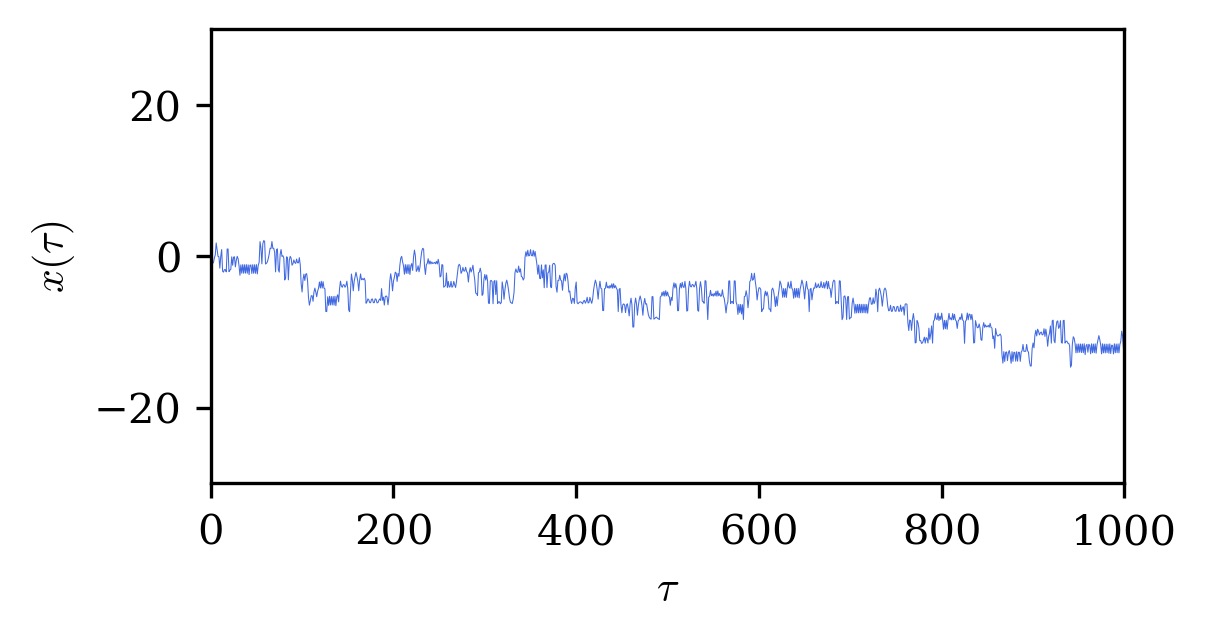
\includegraphics[width = \textwidth]{graf_2ondas/traj_normal.png}
            \caption{Trajectory with normal transport}
        \end{subfigure}
        \begin{subfigure}[b]{0.45\textwidth}
            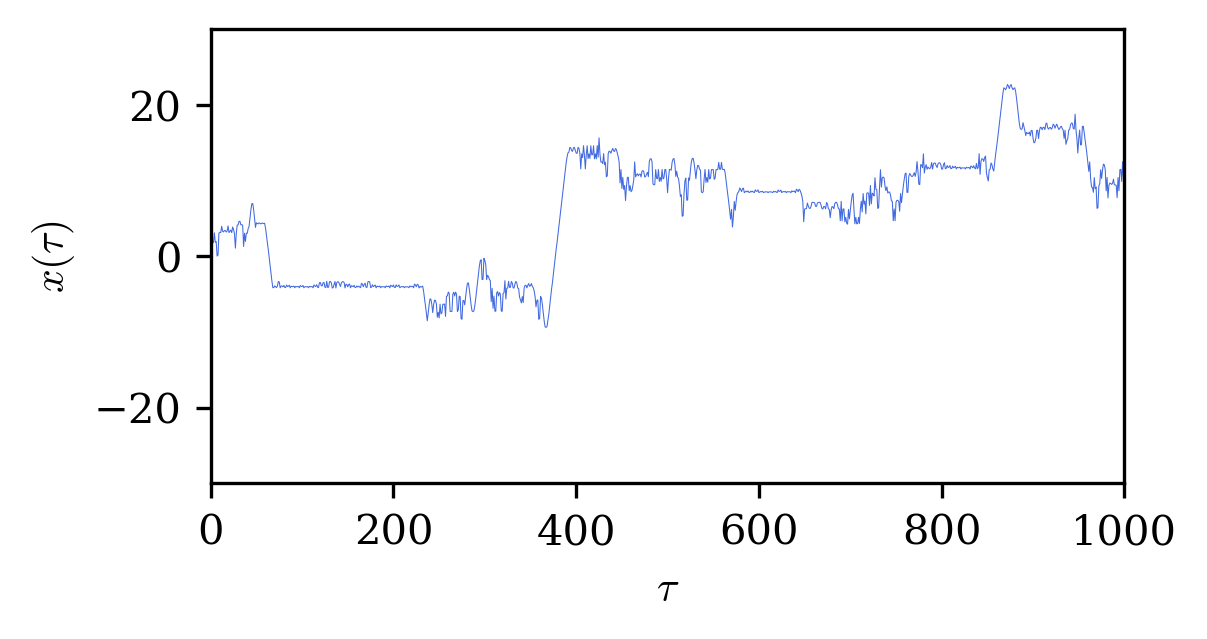
\includegraphics[width = \textwidth]{graf_2ondas/traj_anom.png}
            \caption{Duperdiffusive Trajectory}
        \end{subfigure}

        \caption{General Trajectory behavior}
    \end{figure}
\end{frame}

\begin{frame}{Extras - continuous time system - phase space}
    \begin{equation}
        H(x,y,t) = \phi_o - v_1x + A_1 \sin(k_{x1}x)\cos(k_{y1}y) + \underset{\uparrow}{A_2}\sin(k_{x2}x + \underset{\uparrow}{\theta_x})\cos(k_{y2}(y - vt)).
      \end{equation}
    

    \begin{figure}
        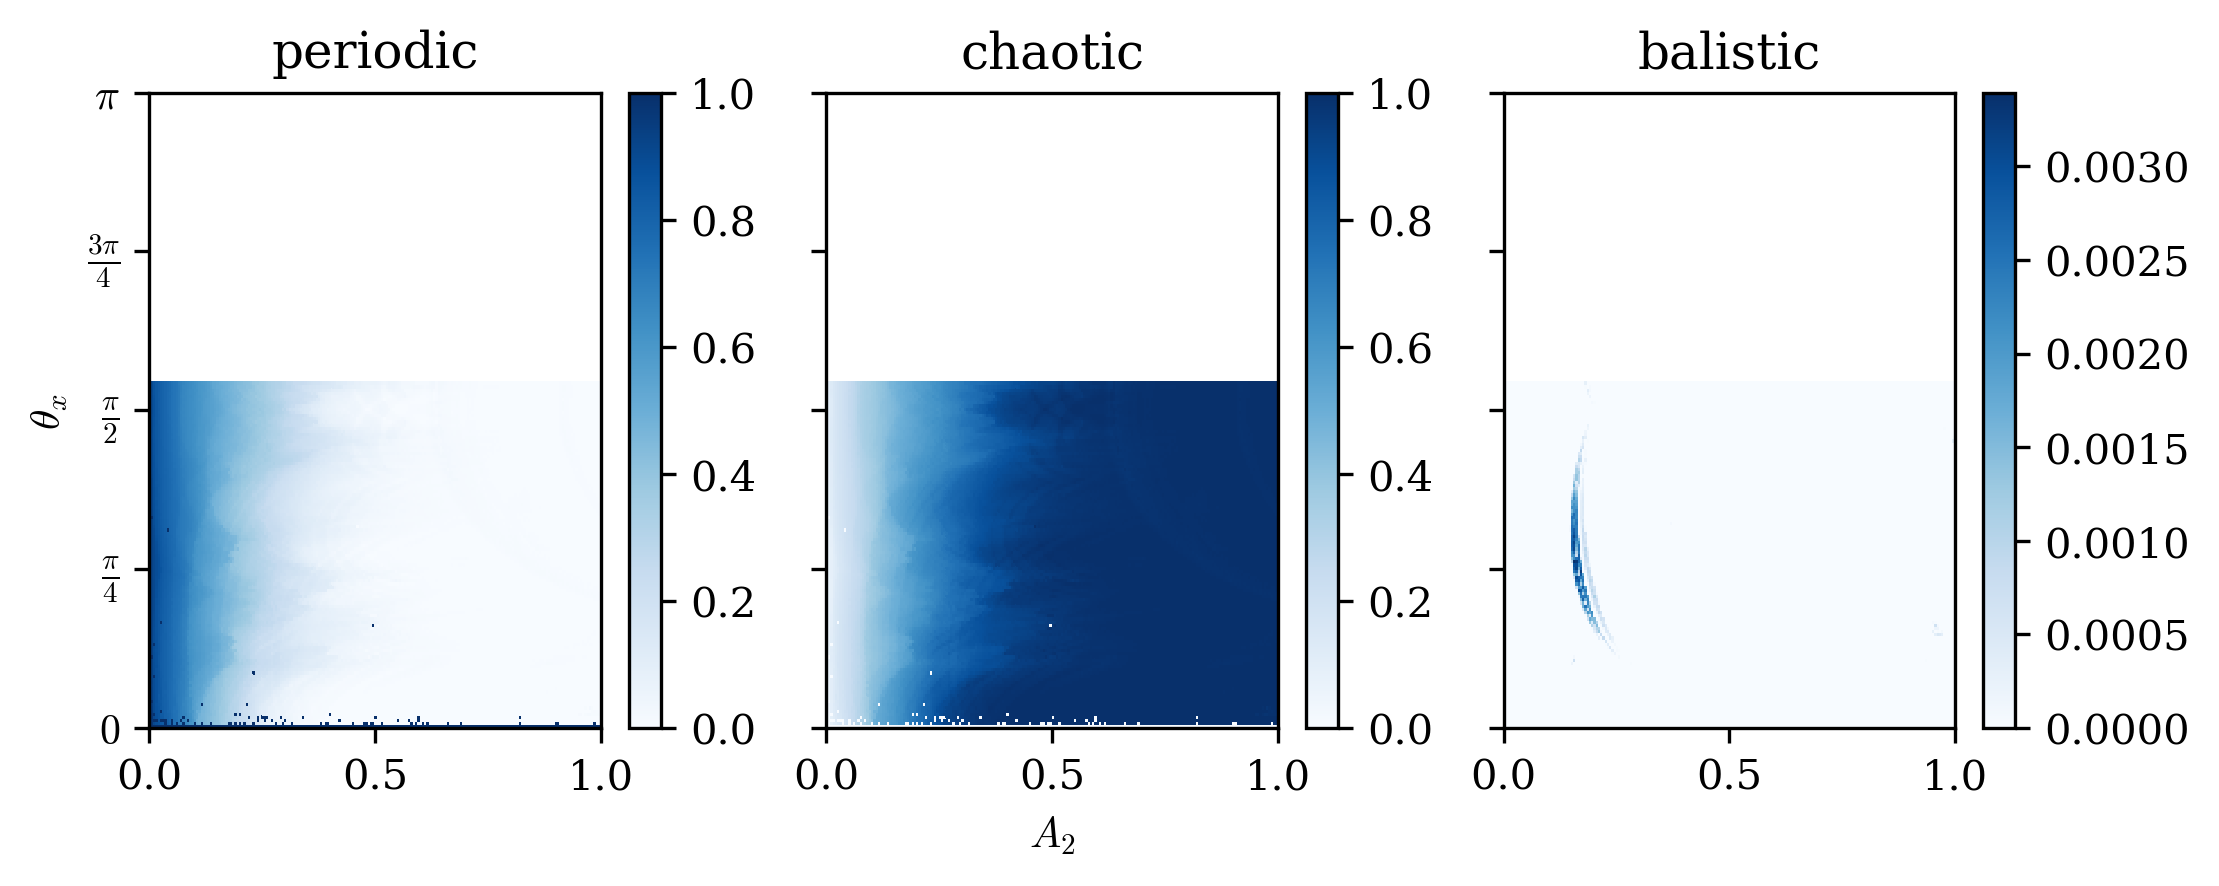
\includegraphics[width = \textwidth]{graf_2ondas/paramspace.png}
        \caption{Categorized regions; Estimated total wall clock simulation time: 20 days with 64 core parallelization on Intel Xeon Gold 5118 at 2.3 GHz}
    \end{figure}
\end{frame}

\begin{frame}{Operations required for different methods}
    \begin{table}
        \begin{tabular}{c|c|c|c}
                &  Detailed displacement & $\gamma$ evaluation & Segment and test\\
            \hline
            Parameters & $N_x \times N_y \times N_{it}$ & $N \times N_{it}$ & $N \times N_{it}$\\
            \hline
            Order & $10^{3} \times 10^{3} \times 10^{2}$  & $10^3 \times 10^4$ & $10^2 \times 10^4$\\
            \hline
            Order & $10^{8}$ & $10^{7}$ & $10^6$\\ 
        \end{tabular}
        \caption{Approximated iterations of some methods to identify anomalous transport}
    \end{table}
\end{frame}
    
    


\end{document}
